\section{Callbacks}

\subsection{Model Checkpoint}
Eğitim sırasında modelin belirli aralıklarla kaydedilmesini sağlar.

\begin{lstlisting}[language=Python]
from keras.callbacks import ModelCheckpoint

checkpoint = ModelCheckpoint(filepath='best_model.h5',
							monitor='val_accuracy',
							verbose=1,
							save_best_only=True,
							mode='max')
\end{lstlisting}

\subsubsection{Hiperparametreler}
\begin{table}[h]
\centering
{\scriptsize\renewcommand{\arraystretch}{0.4}
{\resizebox*{\linewidth}{0.4\textwidth}{
\begin{tabular}{|p{2cm}|p{6cm}|}
\hline
Parametre & Açıklama \\ \hline
filepath & Kaydedilecek dosyanın yolu. \\ \hline
monitor & İzlenecek metriğin adı. \\ \hline
verbose & Çıktı durumu. \\ \hline
save\_best\_only & Sadece en iyi performans gösterdiği durumları kaydet. \\ \hline
mode & Monitor metriğinin neye göre değerlendirileceği. "max" veya "min". \\ \hline
period & Kaydetme aralığı. \\ \hline

\end{tabular}
}}}
\end{table}

\subsection{BackupAndRestore}
Eğitim sırasında modelin yedeklerini alarak ve geri yükleyerek eğitim sırasında oluşabilecek herhangi bir kesintiden sonra eğitimin devam etmesini sağlar.

\begin{lstlisting}[language=Python]
from keras.callbacks import BackupAndRestore

backup = BackupAndRestore(backup_dir,
						 save_freq="epoch")
\end{lstlisting}

\subsubsection{Hiperparametreler}
\begin{table}[h]
\centering
{\scriptsize\renewcommand{\arraystretch}{0.4}
{\resizebox*{\linewidth}{0.1\textwidth}{
\begin{tabular}{|p{2cm}|p{6cm}|}
\hline
Parametre & Açıklama \\ \hline
backup\_dir & Yedekleme dizini. \\ \hline
frequency & Yedekleme sıklığı. \\ \hline

\end{tabular}
}}}
\end{table}

\subsection{TensorBoard}
Tensorflow'un görselleştirme aracıdır ve modelin performansını izlemek, hata analizi yapmak ve eğitim sürecini anlamak için kullanılır.

\begin{lstlisting}[language=Python]
from keras.callbacks import Tensorboard

tensorboard_callback = TensorBoard(log_dir='./logs')
\end{lstlisting}

\subsubsection{Hiperparametreler}
\begin{table}[h]
\centering
{\scriptsize\renewcommand{\arraystretch}{0.4}
{\resizebox*{\linewidth}{0.2\textwidth}{
\begin{tabular}{|p{2cm}|p{6cm}|}
\hline
Parametre & Açıklama \\ \hline
log\_dir & Log kaydedileceği dizin. \\ \hline
histogram\_freq & Histogram güncelleme sıklığı. \\ \hline
write\_graph & Model grafiğinin tensorboard'da gösterilmesi \\ \hline
write\_images & Modelin görsel tanımının tensorboard'da gösterilmesi. \\ \hline

\end{tabular}
}}}
\end{table}

\subsection{EarlyStopping}
Belirli bir metriği izleyerek iyileşmediği durumlarda eğitimi durdurur. Bu, overfitting durumlarında eğitimi sonlandırmak için kullanılır.

\begin{lstlisting}[language=Python]
from keras.callbacks import EarlyStopping

early_stopping = EarlyStopping(monitor='val_loss', patience=5)
\end{lstlisting}

\subsubsection{Hiperparametreler}
\begin{table}[h]
\centering
{\scriptsize\renewcommand{\arraystretch}{0.4}
{\resizebox*{\linewidth}{0.2\textwidth}{
\begin{tabular}{|p{2cm}|p{6cm}|}
\hline
Parametre & Açıklama \\ \hline
monitor & Takip edilen metrik. \\ \hline
patience & İzlenecek epoch sayısı. \\ \hline
mode & Değerlendirme türü "min" veya "max". \\ \hline
baseline & Eğitimin durdurulması için belirli bir referans değeri. \\ \hline
restore\_best\_weights & En iyi modelin ağırlıklarını geri yükleme. \\ \hline

\end{tabular}
}}}
\end{table}

\subsection{LearningRateScheduler}
Belirli bir metriği izleyerek iyileşmediği durumlarda eğitimi durdurur. Bu, overfitting durumlarında eğitimi sonlandırmak için kullanılır.

\begin{lstlisting}[language=Python]
from keras.callbacks import LearningRateScheduler

def lr_schedule(epoch, lr): 
	if epoch < 10:
		return lr
	else:
		return lr * np.exp(-0.5)

lr_scheduler = LearningRateScheduler(schedule=lr_scheduler)
\end{lstlisting}

\subsection{ReduceLROnPlateau}
Eğitim sırasında belirli bir metriği iyileşmediği durumlarda öğrenme oranını düşürmek için kullanılır.

\begin{lstlisting}[language=Python]
from keras.callbacks import ReduceLROnPlateau

lr_plat = ReduceLROnPlateua(monitor='val_loss', patience=3, factor=0.2)
\end{lstlisting}

\subsubsection{Hiperparametreler}
\begin{table}[h]
\centering
{\scriptsize\renewcommand{\arraystretch}{0.4}
{\resizebox*{\linewidth}{0.2\textwidth}{
\begin{tabular}{|p{2cm}|p{6cm}|}
\hline
Parametre & Açıklama \\ \hline
monitor & Takip edilecek metrik adı. \\ \hline
factor & Öğrenme oranını azaltmak için çarpan. \\ \hline
patience & İzlenecek epoch sayısı. \\ \hline
mode & Değerlendirme türü. \\ \hline
cooldown & Öğrenme oranını azalttıktan sonra bekleyeceği epoch sayısı. \\ \hline

\end{tabular}
}}}
\end{table}

\subsection{CSVLogger}
Eğitim sırasında modelin metriklerini bir CSV dosyasına kaydeder.

\begin{lstlisting}[language=Python]
from keras.callbacks import CSVLogger

csv_log = CSVLogger(filename='file.csv', seperator=',')
\end{lstlisting}

\newpage

\section{Conv}
\textbf{Conv1D:} 1 boyutlu konvolüsyon işlemi uygulamak için kullanılan bir katmandır. Giriş verileri üzerinde belirli bir pencere boyutunda kaydırılan bir filtre (kernel) uygular. Bu filtre, giriş verilerini bir boyutlu konvolüsyon işleminden geçirir ve çıktı olarak konvolüsyon sonuçlarını verir. Genellikle zamansal verilerin işlenmesi, sıralı verilerin analizi gibi durumlarda kullanılır.\\
\textbf{Conv2D:} 2 boyutlu konvolüsyon işlemi uygulamak için kullanılan bir katmandır. Giriş verileri üzerinde belirli bir pencere boyutunda kaydırılan bir filtre (kernel) uygular. Bu filtre, giriş verilerini iki boyutlu konvolüsyon işleminden geçirir ve çıktı olarak konvolüsyon sonuçlarını verir. Genellikle görüntü işleme gibi iki boyutlu verilerin işlenmesi durumlarda kullanılır. \\
\textbf{Conv3D:} 3 boyutlu konvolüsyon işlemi uygulamak için kullanılan bir katmandır. Giriş verileri üzerinde belirli bir pencere boyutunda kaydırılan bir filtre (kernel) uygular. Bu filtre, giriş verilerini üç boyutlu konvolüsyon işleminden geçirir ve çıktı olarak konvolüsyon sonuçlarını verir. Genellikle video işleme, 3D görüntü verileri gibi üç boyutlu verilerin işlenmesi durumlarda kullanılır.

\begin{figure}[h]
    \centering
    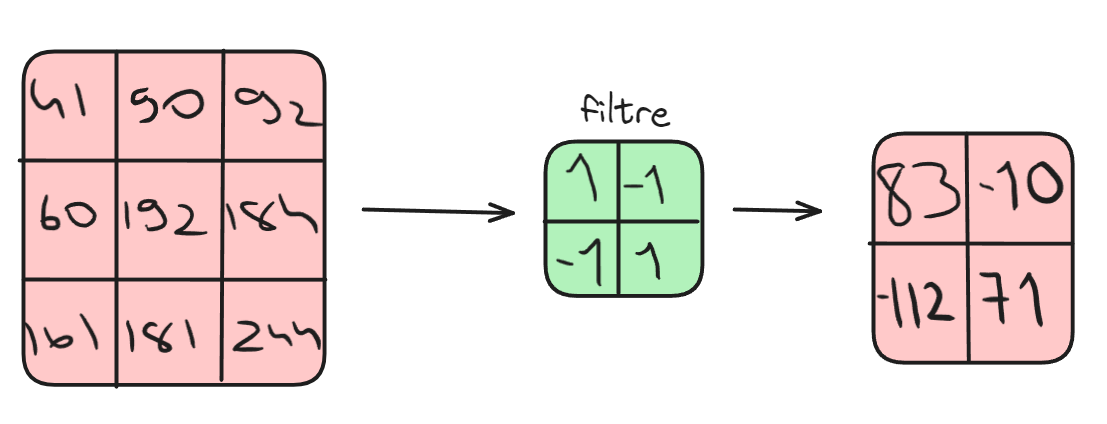
\includegraphics[width=0.7\textwidth]{images/conv_layer.png}
    \caption{Konvolüsyon katmanı.}
    \label{fig:enter-label}
\end{figure}

\subsubsection{Hiperparametreler}
\begin{table}[h]
\centering
{\scriptsize\renewcommand{\arraystretch}{0.4}
{\resizebox*{\linewidth}{0.2\textwidth}{
\begin{tabular}{|p{2cm}|p{6cm}|}
\hline
Parametre & Açıklama \\ \hline
filters & Çıkış uzayının boyutu. \\ \hline
kernel\_size & Filtre boyutu. \\ \hline
stride & Kaydırma adımı \\ \hline
padding & Giriş boyutunu ayarlamak için kullanılcak yöntem. \\ \hline
activation & Aktivasyon fonksiyonu. \\ \hline

\end{tabular}
}}}
\end{table}

\newpage